\documentclass[]{standalone}

\usepackage{../lenses}

\begin{document}
 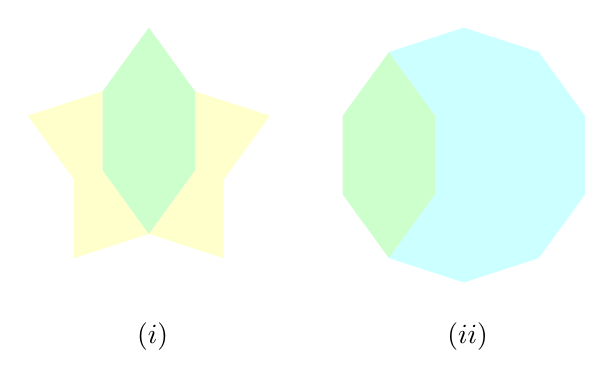
\begin{tikzpicture}
  \begin{scope}[scale=1]
   \definecolor{leaf}{HTML}{CCFFCC} % green
   \definecolor{moon}{HTML}{CCFFFF} % cyan
   \definecolor{crown}{HTML}{FFFFCC} % yellow
   \pgfmathsetmacro\side{1}
   \pgfmathsetmacro\a{180/5}
   \pgfmathsetmacro\ca{\side*cos(\a)}
   \pgfmathsetmacro\sa{\side*sin(\a)}
   \pgfmathsetmacro\cb{\side*cos(2*\a)}
   \pgfmathsetmacro\sb{\side*sin(2*\a)}
   \pgfmathsetmacro\cc{\side*cos(3*\a)}
   \pgfmathsetmacro\sc{\side*sin(3*\a)}
   
   \begin{scope}[shift={(0,-1)}] % decagonal star
    \begin{scope}[rotate=180/10]
     \fill[crown] (0,0) % C+C
      -- ++(-\cc,\sc)
      -- ++(\cc,\sc)
      -- ++(\side,0)
      -- ++(\cc,-\sc)
      -- ++(\cb,-\sb)
      -- ++(\ca,\sa)
      -- ++(-\cc,\sc)
      -- ++(\ca,-\sa)
      -- ++(-\ca,-\sa)
      -- ++(\cc,-\sc)
      -- ++(-\ca,\sa)
      -- cycle;
      \fill[leaf] (\side,0)
       -- ++(\cc,\sc)
       -- ++(-\cc,\sc)
       -- ++(\ca,\sa)
       -- ++(-\cc,-\sc)
       -- ++(\cc,-\sc)
       -- cycle;
     \lenseC{000000}{\side}{1}
     \begin{scope}[shift={(\side,0)},rotate=36] \lenseB{000000}{\side}{1} \end{scope}    
     \begin{scope}[shift={(\side,0)},rotate=-36] \lenseC{000000}{\side}{1} \end{scope}    
    \end{scope}
    \draw (1,-1) node{$(i)$};
   \end{scope}
   
   \begin{scope}[shift={(4,-1)}] % regular decagon
    \begin{scope}[rotate=3*180/10]
    \fill[leaf] (0,0)
     -- ++(\cb,\sb)
     -- ++(\ca,\sa)
     -- ++(\side,0)
     -- ++(-\cb,-\sb)
     -- ++(-\ca,-\sa)
     -- cycle;
     \lenseB{000000}{\side}{1}
     
     \fill[moon] (\side,0)
     -- ++(\ca,\sa)
     -- ++(\cb,\sb)
     -- ++(\ca,-\sa)
     -- ++(-\cc,-\sc)
     -- ++(\cc,-\sc)
     -- ++(-\ca,-\sa)
     -- ++(-\side,0)
     -- ++(-\ca,\sa)
     -- ++(-\cb,\sb)
     -- cycle;
     
     \begin{scope}[rotate=-72] \lenseB{000000}{\side}{1} \end{scope}   
     \begin{scope}[shift={(\side,0)},rotate=-36] \lenseC{000000}{\side}{1} \end{scope}   
     \begin{scope}[shift={(\side,0)},rotate=-36]
      \begin{scope}[shift={(\side,0)},rotate=-36]
       \begin{scope}[shift={(\side,0)},rotate=-36+144]
        \lenseB{000000}{\side}{1}
       \end{scope}
      \end{scope}
     \end{scope}   
    \end{scope}   
    \draw (1,-1) node{$(ii)$};
   \end{scope}
  
  \end{scope}
 \end{tikzpicture}
\end{document}